Anomalous isolated energy deposits with reconstructed energies that can exceed 100~GeV have been observed in the ECAL.
These deposits, commonly referred to as \emph{spikes}, occur at a rate proportional to the collision rate and can create significant challenges for triggering at high luminosity.
If not rejected, spikes can bias the reconstructed energies and times of electrons, photons, jets, and the missing transverse momentum in an event.
In the ECAL barrel, spikes originate primarily from particles directly striking the avalanche photodiodes (APDs), producing large signals through direct ionization in the silicon sensor~\cite{Petyt:2012upa}.
Spike energy is typically concentrated in a single crystal and is characterized by a fast-rising pulse shape with little or no scintillation component.
In most cases there is minimal activity in neighboring crystals, although occasional ``double spikes'' produce spike-like signals in two adjacent crystals.
A reconstructed hit (rechit) produced by a spike is referred to as a \emph{spike rechit}.

The performance of standard spike-rejection flags is studied in the context of the CC timing reconstruction.
For this study, rechit collections are produced for both the ratio and CC timing methods and stored directly as output of the corresponding reconstruction modules, without downstream cleaning, filtering, or timing calibration.
The CC reconstruction is performed without the OOT amplitude correction to minimize time-dependent effects arising from the energy reconstruction.
These collections are referred to as \emph{raw} rechit collections.

\begin{figure}[h!tbp]
\begin{center}
\resizebox{0.75\textwidth}{!}{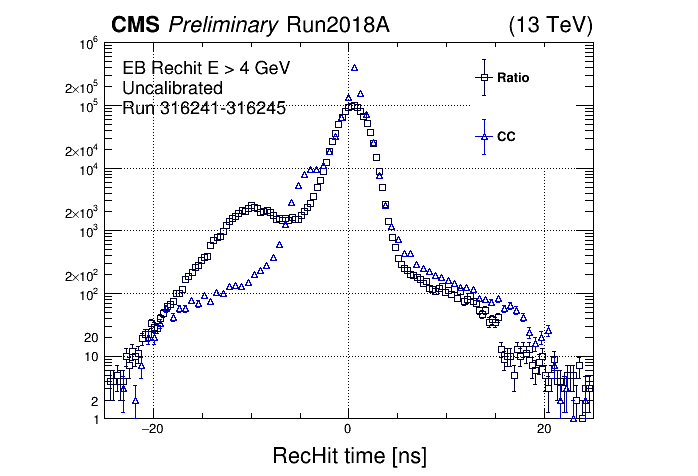
\includegraphics{fig/sec_gen/tr_hl_spike_distro_10062022142744.png}}
\caption{Distribution of rechit times reconstructed with the ratio method and the CC method for rechits with energy $>4$~GeV, using raw rechit collections saved without downstream cleaning, filtering, or calibration.
Secondary structures at approximately $-10$~ns (ratio) and $-5$~ns (CC) are dominated by spike rechits.}
\label{raw_distro}
\end{center}
\end{figure}

Figure~\ref{raw_distro} shows the rechit time distributions in the raw collections for rechits with energy greater than 4~GeV.
Secondary structures are observed at approximately $-10$~ns for the ratio method and $-5$~ns for the CC method; these features are dominated by spike rechits.
Figure~\ref{2d_raw_distro_comp} shows the correlation between the raw CC and ratio rechit times for rechits with energies between 10 and 120~GeV.
A strong correlation is observed between the reconstructed times obtained with the two methods, while the CC method exhibits a narrower prompt-time population.
In this sample, spike rechits populate an early-time region spanning approximately $-6$ to $-15$~ns for the ratio method and $-2$ to $-10$~ns for the CC method.

\begin{figure}[h!tbp]
\begin{center}
\resizebox{0.7\textwidth}{!}{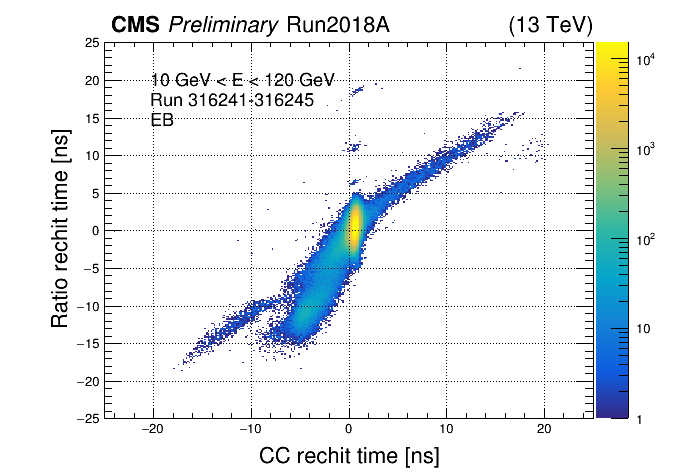
\includegraphics{fig/sec_gen/tr_2d_RtvCC_spike_10062022125336.png}}
\caption{Correlation of raw rechit times reconstructed with the CC method and the ratio method for rechits with energies between 10 and 120~GeV.
The CC method exhibits a narrower prompt-time population.
Spike rechits populate an early-time region at approximately $-6$ to $-15$~ns for the ratio method and $-2$ to $-10$~ns for the CC method.}
\label{2d_raw_distro_comp}
\end{center}
\end{figure}

Spike rechits are characterized by reconstructed times that are significantly earlier than those of scintillation-induced signals.
For spike-like pulse shapes, the fast rise time biases the ratio-based timing reconstruction toward earlier times.
The CC method is less sensitive to this effect and yields a smaller, though still non-negligible, early-time bias.
In addition, spike rechits are typically isolated from surrounding activity.
Since isolated high-energy deposits are inconsistent with electromagnetic shower development, spike rejection can exploit both the topology of local energy sharing and the reconstructed time.

The swiss-cross variable characterizes the degree of energy sharing between a crystal with a large deposit and its nearest neighbors, with values closer to one indicating a more isolated deposit.
The swiss-cross is used to define topological spike-rejection flags, including \texttt{kWeird}, which rejects isolated energy deposits, and \texttt{kDiWeird}, which targets double spikes~\cite{Petyt:2012upa}.
In addition, a timing-based rechit flag \texttt{kOutOfTime} (\texttt{kOOT}) is defined using energy-dependent time thresholds that may be configured separately for the barrel and endcaps and for different energy ranges.
This flag defines a time window around the prompt population and marks rechits reconstructed outside this window on either the early or delayed side.

\begin{figure}[h!tbp]
\begin{center}
\resizebox{0.375\textwidth}{!}{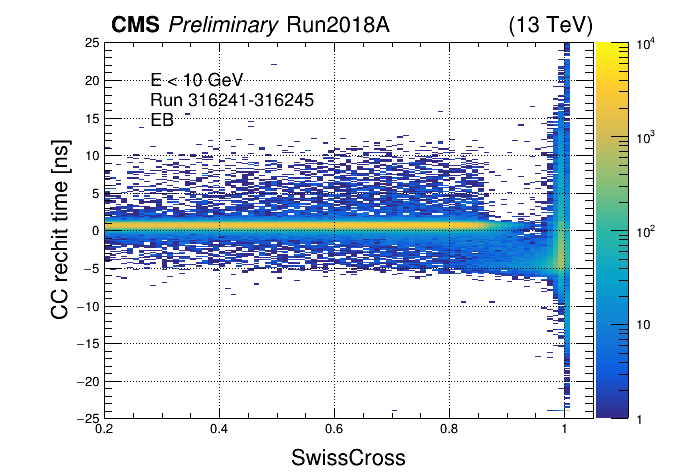
\includegraphics{fig/sec_gen/tr_2d_CC_swisscross1_10062022134628.png}}
\resizebox{0.375\textwidth}{!}{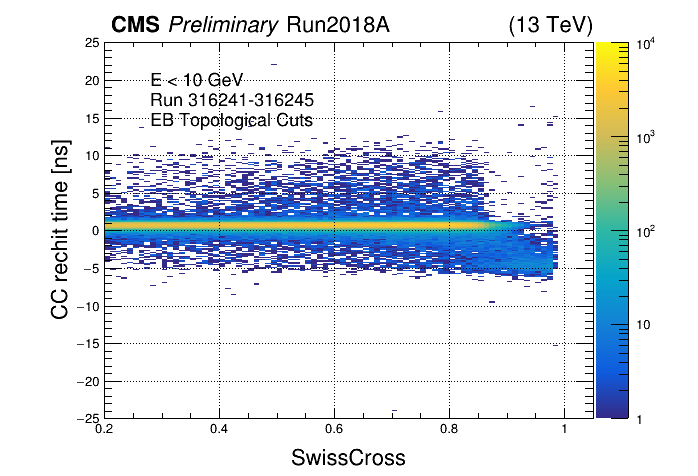
\includegraphics{fig/sec_gen/tr_2d_CC_swisscross2_10062022134846.png}}
\resizebox{0.375\textwidth}{!}{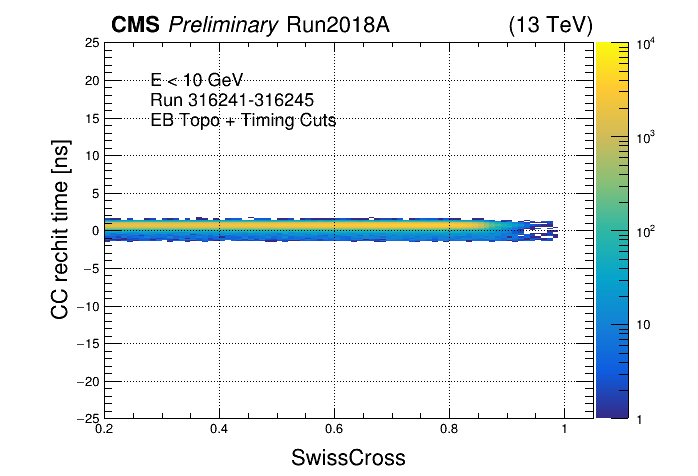
\includegraphics{fig/sec_gen/tr_2d_CC_swisscross3_10062022135015.png}}
\caption{Swiss-cross as a function of CC reconstructed rechit time for rechits with energy $>10$~GeV.
Left: distribution without spike-rejection cuts, showing a prompt population and a spike-dominated population at large swiss-cross values and early reconstructed times.
Middle: distribution after applying the topological spike-rejection flags (\texttt{kWeird} and \texttt{kDiWeird}), where most spike rechits are removed, though a residual early-time feature remains.
Right: distribution after additionally applying the \texttt{kOOT} timing flag using a 3~ns threshold for all timing parameters, where the remaining spike population is strongly suppressed.}
\label{swisscross_CC}
\end{center}
\end{figure}

A rechit flagged as \texttt{kOOT} is unlikely to be used in downstream particle reconstruction, and overly aggressive timing thresholds can therefore reduce the reconstructed energy of physics objects.
It is consequently necessary to tune the \texttt{kOOT} thresholds for the CC time reconstruction to maximize spike rejection while minimizing impact on prompt scintillation signals across the full rechit energy range.
Since CC reconstructed times exhibit a different energy dependence than ratio reconstructed times, the optimal \texttt{kOOT} parameter values for low- and high-energy rechits must be determined independently.

Based on these studies, the \texttt{kOOT} timing thresholds for the CC reconstruction are tuned to achieve efficient rejection of spike rechits while preserving prompt scintillation signals across the full rechit energy range.
Separate threshold values are optimized for low- and high-energy rechits to account for the energy dependence of the CC reconstructed time.
The selected parameter configuration provides strong suppression of spike-induced early-time populations with minimal impact on downstream particle reconstruction.
Unless otherwise stated, this tuned \texttt{kOOT} configuration is used for the CC timing reconstruction in all subsequent performance studies presented in this paper.
